\documentclass{article}
\usepackage[T1]{fontenc}
\usepackage[utf8]{inputenc}
\usepackage{amssymb}
\usepackage{pythonhighlight}
\usepackage{tikz}
\usepackage{amsmath}
\usepackage[a4paper, left=40mm, right=40mm, top=30mm, bottom=30mm]{geometry}
\usepackage[indent=0pt]{parskip}
\usepackage[backend=biber]{biblatex}
\usepackage{graphicx}
\usepackage{subfig}
\usepackage{subcaption}
\usepackage{float}
\graphicspath{ {../charts/} {../images/} }
\addbibresource{interpolation.bib}

\title{Metody numeryczne - projekt 3 - Aproksymacja profilu wysokościowego}
\author{Jerzy Szyjut, numer albumu: 193064}
\date{19.05.2024r.}

\usepackage{csquotes}
\begin{document}

\maketitle

\begin{section}{Wstęp}
  \subsection{Czym jest interpolacja?}
  Interpolacja to proces przybliżania funkcji, która jest zdefiniowana na dyskretnym zbiorze punktów. 
  W wyniku interpolacji otrzymujemy funkcję, która jest ciągła i przechodzi przez wybrane punkty z oryginalnego zbioru.
  Interpolacja często poprzedza poprzedza takie algorytmy jak: szukanie minimum funkcji, miejsc zerowych, całkowanie,
  liczenie pochodnych itp.
  \subsection{Interpolacje wielomianowe}\cite{interpolacja_wielomianowa_wiki}
  Interpolacje wielomianowe to rodzaj interpolacji, w której przybliżamy funkcję za pomocą wielomianu.
  Przyjmuje ona wielomian stopnia $n$, który przechodzi przez $n+1$ punktów z oryginalnego zbioru.
  Najprostszym sposobem interpolacji wielomianowej jest interpolacja z użyciem macierzy Vandermonde'a.
  Jednak interpolacja ta, wymaga obliczenia wielu równań liniowych, zarówno zawierających wielkie liczby, jak i
  liczby bliskie zeru. Powoduje to, że metoda ta jest niestabilna numerycznie. Znacznie lepszym sposobem interpolacji
  wielomianowej jest interpolacja Lagrange'a.
  \subsection{Interpolacja Lagrange'a}\cite{wyklad5}
  Interpolacja Lagrange'a to jedna z metod interpolacji wielomianowej. W tej metodzie, przybliżamy funkcję za pomocą
  wielomianu stopnia $n$, który przechodzi przez $n+1$ punktów z oryginalnego zbioru. Baza wielomianów Lagrange'a
  jest zdefiniowana jako:
  \begin{equation}
    fi_{i}(x) = \prod_{j=1, j \neq i}^{n + 1} \frac{(x - x_{j})}{(x_{i} - x_{j})}
  \end{equation}
  dla $i = 1, 2, ..., n + 1$. Wielomian interpolacyjny Lagrange'a jest zdefiniowany jako:
  \begin{equation}
    P(x) = \sum_{i=1}^{n + 1} y_{i}fi_{i}(x)
  \end{equation}
  gdzie $y_{i}$ to wartość funkcji w punkcie $x_{i}$.
  \subsection{Interpolacja funkcjami sklejanymi (spline)}
  Interpolacja funkcjami sklejanymi to rodzaj interpolacji, w której przybliżamy funkcję za pomocą funkcji sklejanych.
  Funkcje sklejane to funkcje, które są wielomianami stopnia $n$ na każdym z przedziałów, na których jest podzielony
  oryginalny zbiór punktów. Funkcje sklejane są ciągłe na całym przedziale.
  Najpopularniejszym rodzajem funkcji sklejanych jest funkcja sklejana trzeciego stopnia i tej funkcji użyjemy w tym
  projekcie. Funkcja sklejana jest zdefiniowana jako:
  \begin{equation}
    F(x) = S_{i}(x)
  \end{equation}
  gdzie $S_{i}(x)$ to funkcja sklejana na przedziale $[x_{i}, x_{i+1}]$. $S_{i}(x)$ jest wielomianem trzeciego stopnia.
  Aby funkcja sklejana była dobrze dopasowana do oryginalnego zbioru punktów, będzie musiała spełnić następujące warunki:
  \begin{itemize}
    \item $S_{j} = f(x_{j})$ dla $j = 0, 1, ..., n - 1$
    \item $S_{j}(x_{j+1}) = S_{j+1}(x_{j+1})$ dla $j = 0, 1, ..., n - 1$
    \item Dla węzłów wewnętrznych $x_{j}$: $S_{j-1}'(x_{j}) = S_{j}'(x_{j})$ dla $j = 1, 2, ..., n - 1$ 
    \item Dla węzłów wewnętrznych $x_{j}$: $S_{j-1}''(x_{j}) = S_{j}''(x_{j})$ dla $j = 1, 2, ..., n - 1$
    \item Na krańcach przedziału: $S_{0}''(x_{0}) = S_{n-1}''(x_{n}) = 0$
  \end{itemize}\cite{wyklad5}
  Postacie funkcji sklejanej i pochodnych funkcji sklejanej:
  \begin{itemize}
    \item $S_{0} = a_{0} + b_{0}(x - x_{0}) + c_{0}(x - x_{0})^{2} + d_{0}(x - x_{0})^{3}$
    \item $S_{0}' = b_{0} + 2c_{0}(x - x_{0}) + 3d_{0}(x - x_{0})^{2}$
    \item $S_{0}'' = 2c_{0} + 6d_{0}(x - x_{0})$
    \item $S_{1} = a_{1} + b_{1}(x - x_{1}) + c_{1}(x - x_{1})^{2} + d_{1}(x - x_{1})^{3}$
    \item $S_{1}' = b_{1} + 2c_{1}(x - x_{1}) + 3d_{1}(x - x_{1})^{2}$
    \item $S_{1}'' = 2c_{1} + 6d_{1}(x - x_{1})$
  \end{itemize}\cite{wyklad5}
  Znalezienie wielomianów $S$ polega na znalezieniu współczynników $a, b, c, d$ dla każdego z przedziałów.
  Wszystkie powyższe równości można uzależnić od współczynnika $c$, a następnie rozwiązać układ równań liniowych.
  Postać macierzowa układu równań:
  \begin{equation}
    \begin{bmatrix}
      1 & 0 & 0 & 0 & 0 & 0 & 0 & 0 \\
      h_{1} & 2(h_{1} + h_{2}) & h_{2} & 0 & 0 \\
      0 & h_{2} & 2(h_{2} + h_{3}) & h_{3} & 0 \\
      0 & 0 & h_{3} & 2(h_{3} + h_{4}) & h_{4} \\
      0 & 0 & 0 & 0 & 1
    \end{bmatrix}
    \begin{bmatrix}
      c_{0} \\
      c_{1} \\
      c_{2} \\
      c_{3} \\
      c_{4}
    \end{bmatrix}
    =
    \begin{bmatrix}
      0 \\
      3(\frac{y_{2} - y_{1}}{h_{1}} - \frac{y_{1} - y_{0}}{h_{0}}) \\
      3(\frac{y_{3} - y_{2}}{h_{2}} - \frac{y_{2} - y_{1}}{h_{1}}) \\
      3(\frac{y_{4} - y_{3}}{h_{3}} - \frac{y_{3} - y_{2}}{h_{2}}) \\
      0
    \end{bmatrix}
  \end{equation}
  gdzie $h_{i} = x_{i+1} - x_{i}$.
  Pozostałe współczynniki $a, b, d$ można znaleźć za pomocą wzorów:
  \begin{itemize}
    \item $a_{i} = y_{i}$
    \item $b_{i} = \frac{y_{i+1} - y_{i}}{h_{i}} - \frac{h_{i}(2c_{i} + c_{i+1})}{3}$
    \item $d_{i} = \frac{c_{i+1} - c_{i}}{3h_{i}}$
  \end{itemize}
  W celu rozwiązania układu równań liniowych użyłem faktoryzacji LU zaimplementowanej w poprzednim projekcie.
\end{section}

\begin{section}{Analiza podstawowa interpolacji wielomianowej pierwszej trasy}
  \begin{figure}[H]
    \centering
    \subfloat{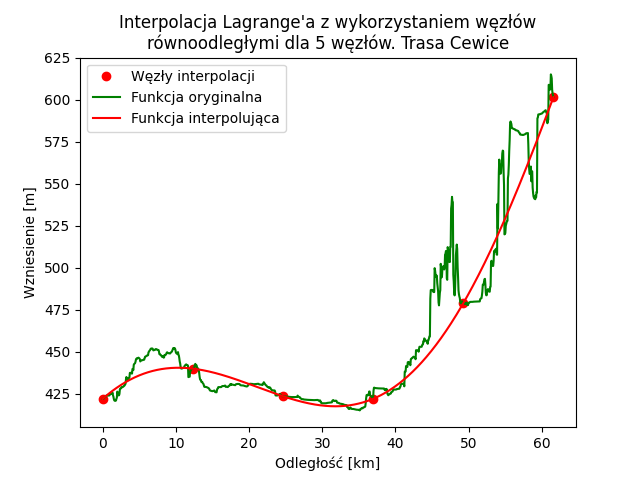
\includegraphics[width=0.5\textwidth]{cewice_l_r_5.png}}
    \subfloat{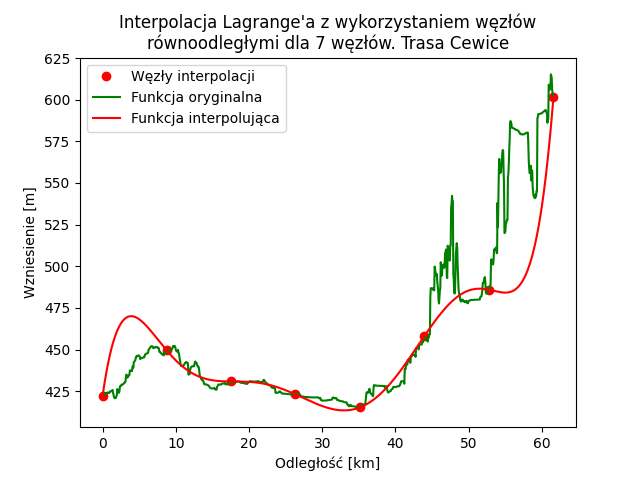
\includegraphics[width=0.5\textwidth]{cewice_l_r_7.png}}
  \end{figure}
  \begin{figure}[H]
    \centering
    \subfloat{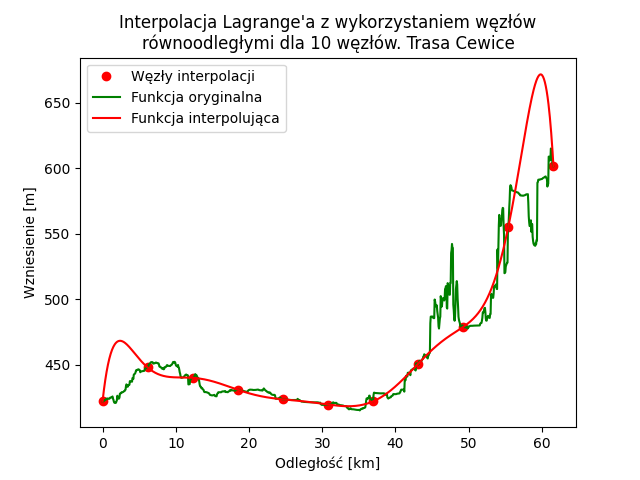
\includegraphics[width=0.5\textwidth]{cewice_l_r_10.png}}
    \subfloat{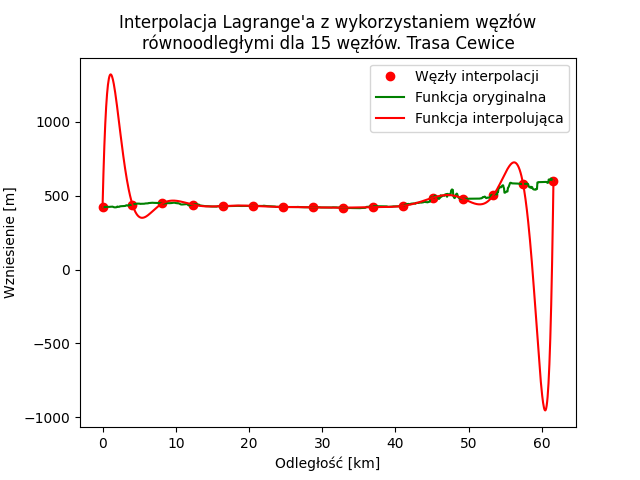
\includegraphics[width=0.5\textwidth]{cewice_l_r_15.png}}
  \end{figure}
  \begin{figure}[H]
    \centering
    \subfloat{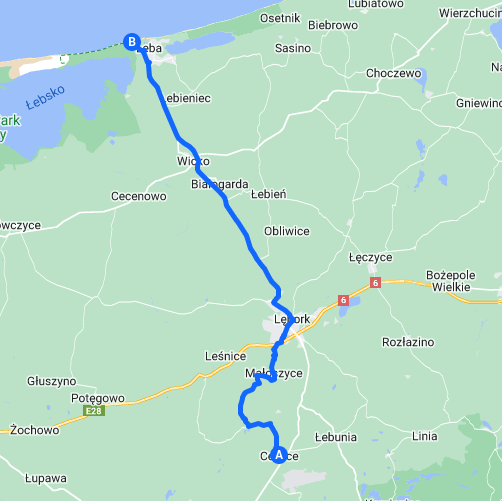
\includegraphics[width=0.5\textwidth]{cewice.png}}
  \end{figure}

  Powyższe wykresu ukazują interpolację pierwszej trasy za pomocą interpolacji wielomianowej Lagrange'a.
  Na wykresach widać, że im większy stopień wielomianu, tym bardziej jest on zbliżony do oryginalnego zbioru punktów.
  Jednak już dla 7 węzłów widać, że na końcach trasy wielomiany zaczynają znacznie odbiegać od oryginalnego zbioru punktów.
  Występuje tu efekt Rungego. Dla 15 węzłów, wielomiany są już bardzo niestabilne i znacznie odbiegają od oryginalnego.
  Skala sprawia, że oryginalny wykres jest prawie płaski.

  Przez częste nieregularności w wysokości trasy, niektóre maksyma i minima lokalne nie są uwzględniane w interpolacji
  przez zbyt małą liczbę węzłów. Widać to na wykresie dla 5 węzłów i 7 węzłów. Nastomiast dla 10 węzłów i 15 węzłów
  zaczyna występować już efekt Rungego. Dla tej trasy ta metoda nie daje najlepszych wyników.
\end{section}

\begin{section}{Analiza podstawowa interpolacji wielomianowej drugiej trasy}
  \begin{figure}[H]
    \centering
    \subfloat{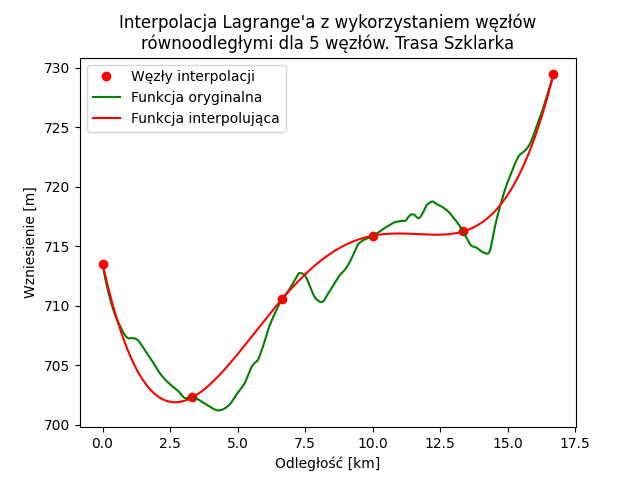
\includegraphics[width=0.5\textwidth]{szklarka_l_r_5.png}}
    \subfloat{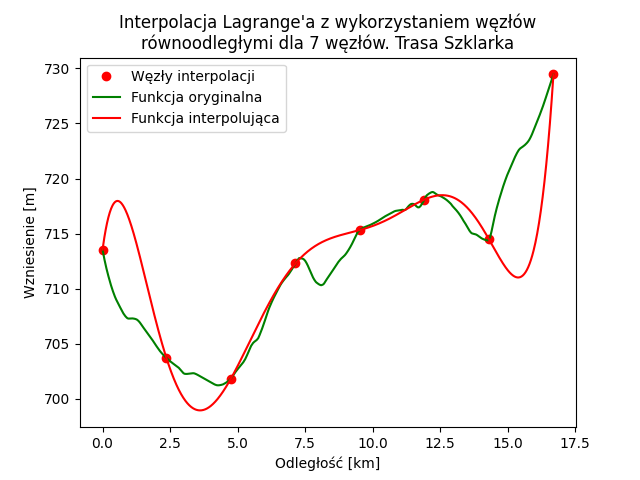
\includegraphics[width=0.5\textwidth]{szklarka_l_r_7.png}}
  \end{figure}
  \begin{figure}[H]
    \centering
    \subfloat{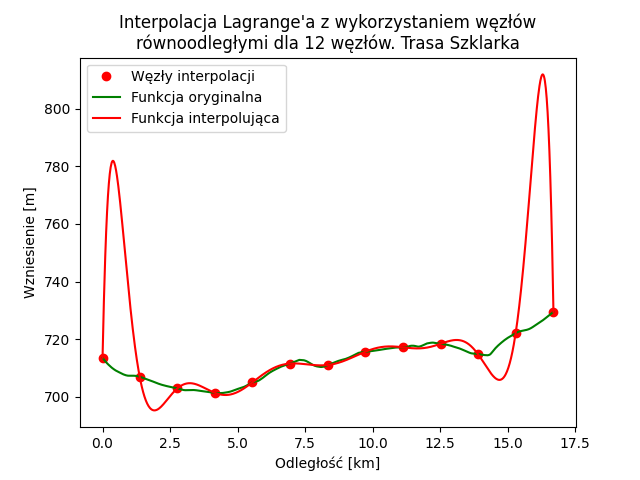
\includegraphics[width=0.5\textwidth]{szklarka_l_r_12.png}}
    \subfloat{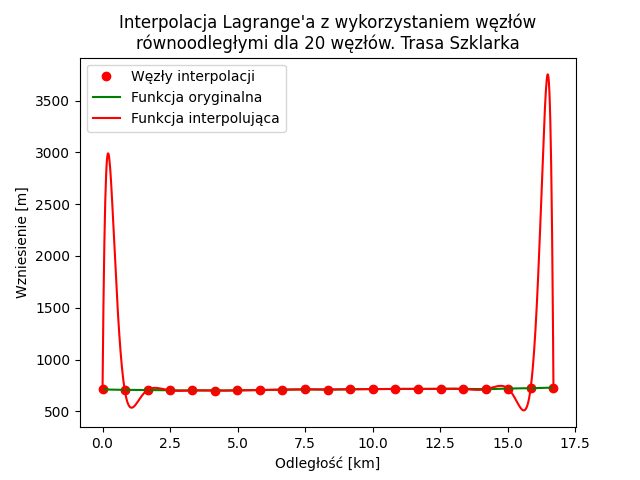
\includegraphics[width=0.5\textwidth]{szklarka_l_r_20.png}}
  \end{figure}
  \begin{figure}[H]
    \centering
    \subfloat{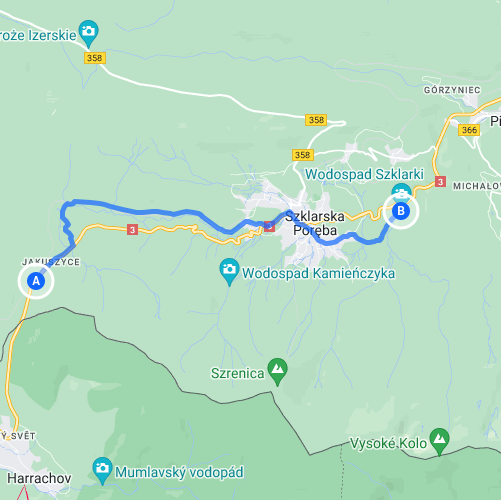
\includegraphics[width=0.5\textwidth]{szklarka.png}}
  \end{figure}

  Powyższe wykresu ukazują interpolację drugiej trasy za pomocą interpolacji wielomianowej Lagrange'a.
  Ze względu na mniejszą nieregularność tej trasy w porównaniu do pierwszej, interpolacja wielomianowa daje lepsze wyniki.
  Zwłaszcza dla 12 węzłów, funkcja jest bardzo zbliżona do oryginalnego zbioru punktów, gdyby nie efekt Rungego.
  Dla 20 węzłów, efekt Rungego jest już bardzo widoczny. Widać, że wielomiany są bardzo niestabilne i znacznie odbiegają
  od oryginalnego zbioru punktów. Po przekalowaniu wykresu, oryginalna trasa jest niemalże linią prostą.
\end{section}

\begin{section}{Analiza dodatkowa interpolacji wielomianowej}
  \subsection{Interpolacja z użyciem węzłów Czebyszewa}\cite{wezly_czebyszewa_wiki}
  Węzły Czebyszewa to węzły, które nie są rozmieszczane równomiernie, ale zgodnie z funkcją Czebyszewa. Funkcja Czebyszewa
  jest zdefiniowana jako:
  \begin{equation}
    x_{i} = cos(\frac{i * pi}{n - 1})
  \end{equation}
  gdzie $i = 0, 1, ..., n - 1$, a $n$ to liczba węzłów. Węzły Czebyszewa są rozmieszczane na przedziale $[-1, 1]$, co wymaga
  dodatkowego przeskalowania węzłów na przedział, na którym interpolujemy funkcję.
  Punkty Czebyszewa są rozmieszczone gęściej na krańcach przedziału, a rzadziej w środku. Dzięki temu, interpolacja z użyciem
  węzłów Czebyszewa przeciwdziała efektowi Rungego.

  \begin{figure}[H]
    \centering
    \subfloat{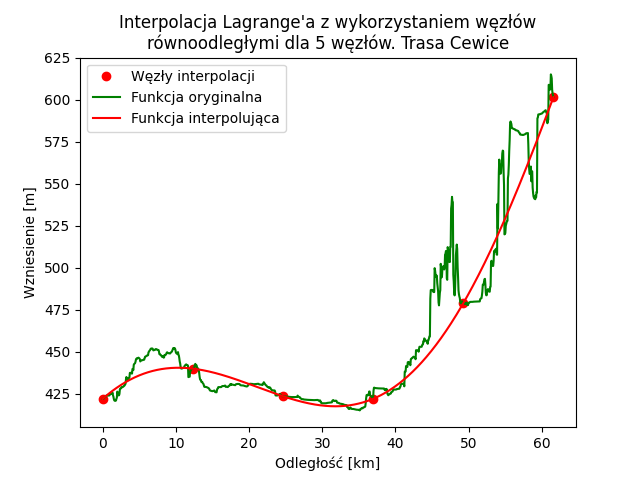
\includegraphics[width=0.5\textwidth]{cewice_l_r_5.png}}
    \subfloat{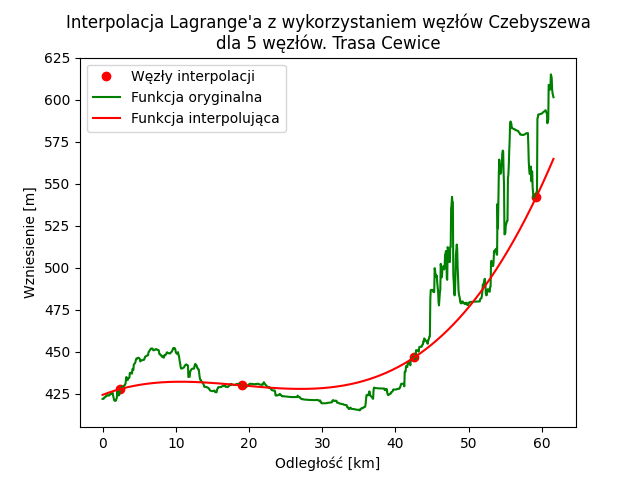
\includegraphics[width=0.5\textwidth]{cewice_l_c_5.png}}
  \end{figure}
  \begin{figure}[H]
    \centering
    \subfloat{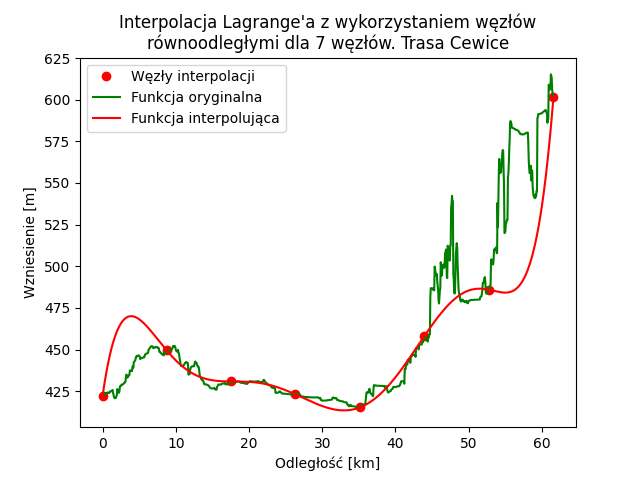
\includegraphics[width=0.5\textwidth]{cewice_l_r_7.png}}
    \subfloat{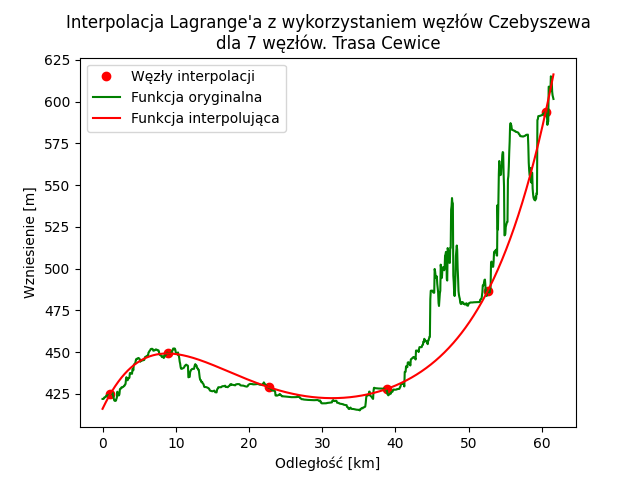
\includegraphics[width=0.5\textwidth]{cewice_l_c_7.png}}
  \end{figure}
  \begin{figure}[H]
    \centering
    \subfloat{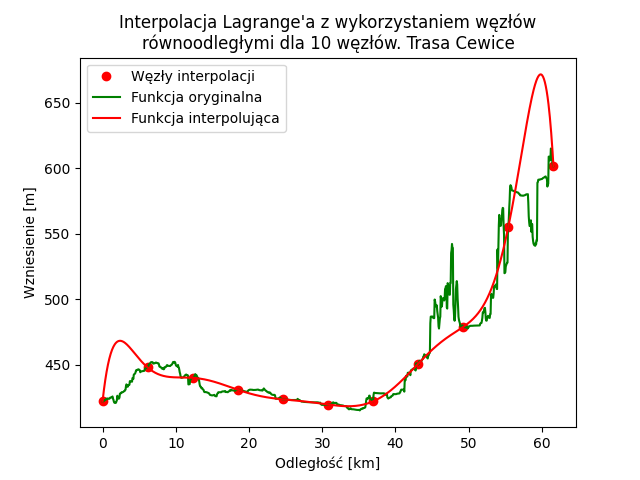
\includegraphics[width=0.5\textwidth]{cewice_l_r_10.png}}
    \subfloat{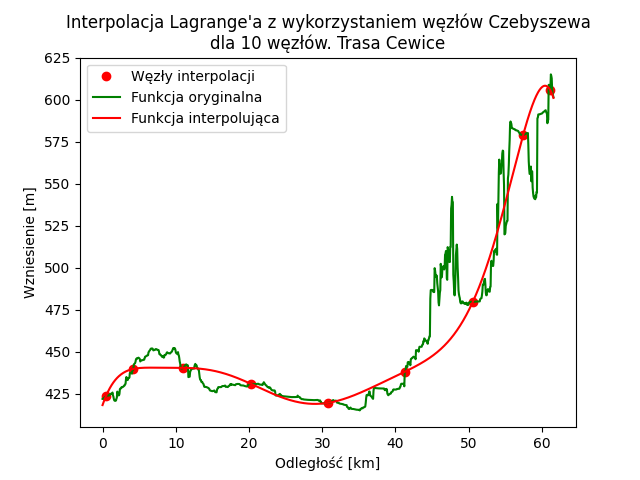
\includegraphics[width=0.5\textwidth]{cewice_l_c_10.png}}
  \end{figure}
  \begin{figure}[H]
    \centering
    \subfloat{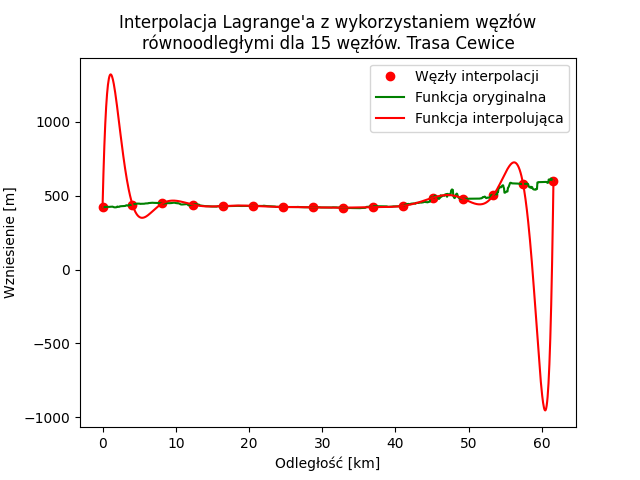
\includegraphics[width=0.5\textwidth]{cewice_l_r_15.png}}
    \subfloat{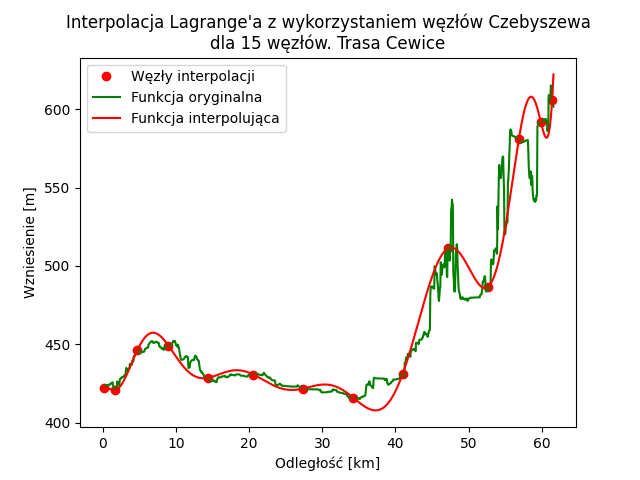
\includegraphics[width=0.5\textwidth]{cewice_l_c_15.png}}
  \end{figure}
  \begin{figure}[H]
    \centering
    \subfloat{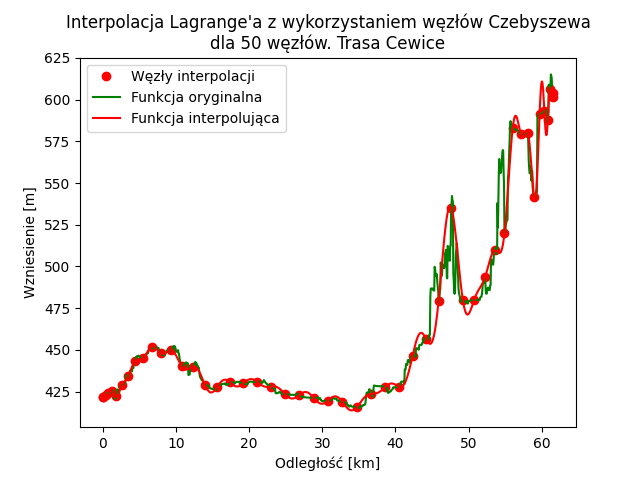
\includegraphics[width=0.5\textwidth]{cewice_l_c_50.png}}
  \end{figure}

  Powyższe wykresy ukazują interpolację pierwszej trasy za pomocą interpolacji wielomianowej Lagrange'a dla tej samej liczby
  węzłów, ale wykresy po prawej stronie nie mają równomiernie rozmieszczonych węzłów, a węzły są rozmieszczone
  przy użyciu funkcji Czebyszewa drugiego rodzaju. Widać, że dla tej samej liczby węzłów, interpolacja z użyciem
  węzłów Czebyszewa daje znacznie lepsze wyniki. Zagęszczenie węzłów w na końcach przedziału pozwala na ogólne
  lepsze dopasowanie wielomianu do oryginalnego zbioru punktów, kosztem większego błędu w środku przedziału.

  Dla 50 węzłów, wielomian jest bardzo zbliżony do oryginalnego zbioru punktów. Dzięki węzłom Czebyszewa, nie uwydatnia
  się efekt Rungego.

  \begin{figure}[H]
    \centering
    \subfloat{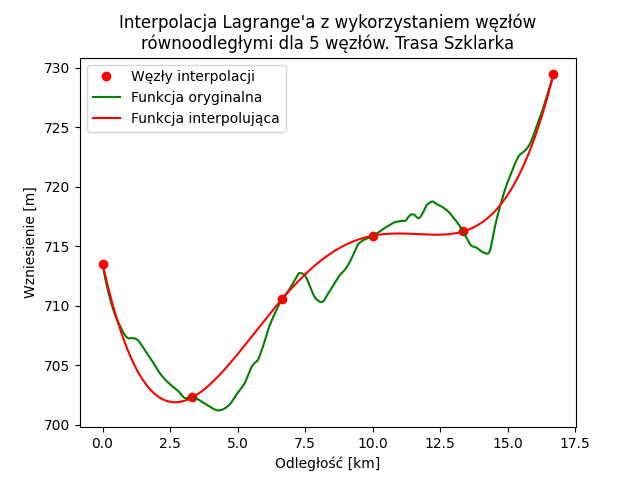
\includegraphics[width=0.5\textwidth]{szklarka_l_r_5.png}}
    \subfloat{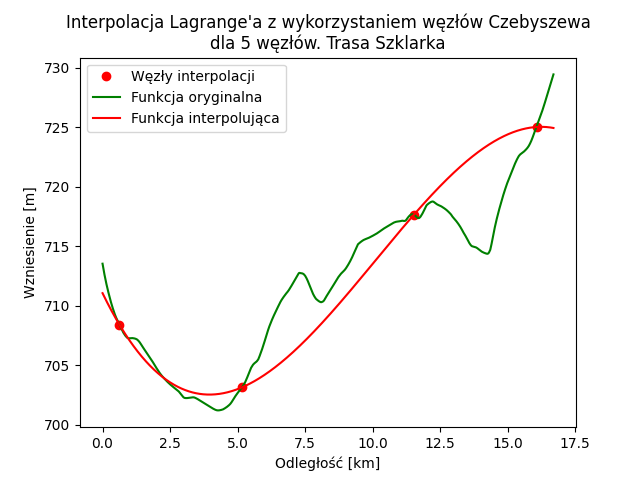
\includegraphics[width=0.5\textwidth]{szklarka_l_c_5.png}}
  \end{figure}
  \begin{figure}[H]
    \centering
    \subfloat{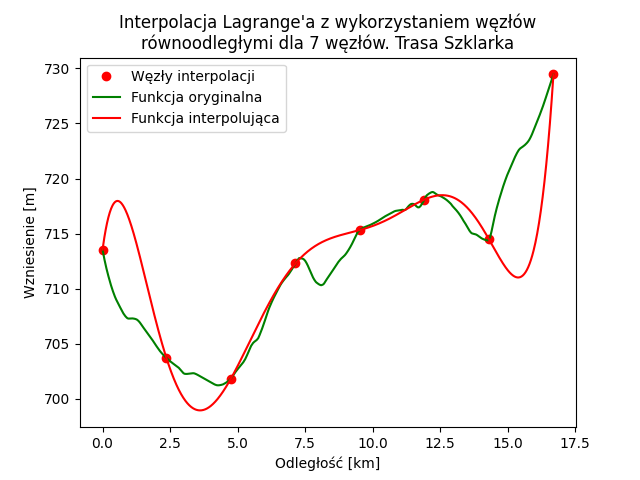
\includegraphics[width=0.5\textwidth]{szklarka_l_r_7.png}}
    \subfloat{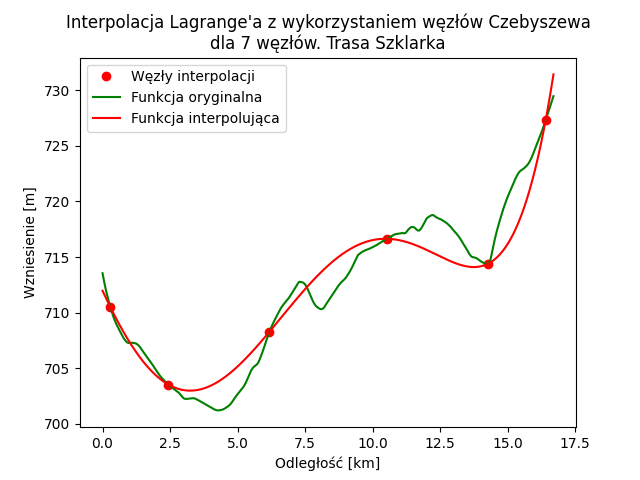
\includegraphics[width=0.5\textwidth]{szklarka_l_c_7.png}}
  \end{figure}
  \begin{figure}[H]
    \centering
    \subfloat{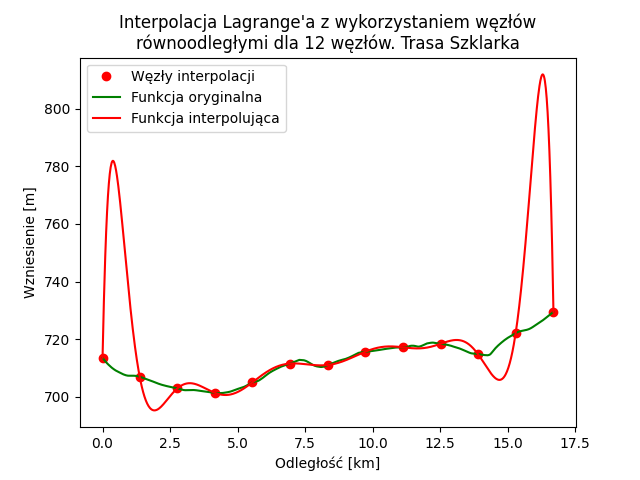
\includegraphics[width=0.5\textwidth]{szklarka_l_r_12.png}}
    \subfloat{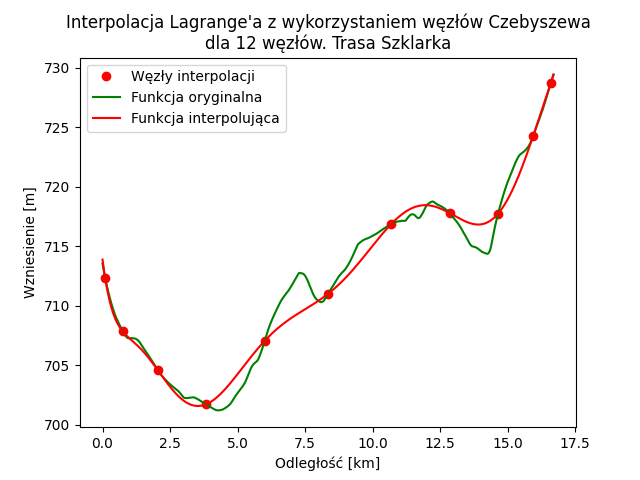
\includegraphics[width=0.5\textwidth]{szklarka_l_c_12.png}}
  \end{figure}
  \begin{figure}[H]
    \centering
    \subfloat{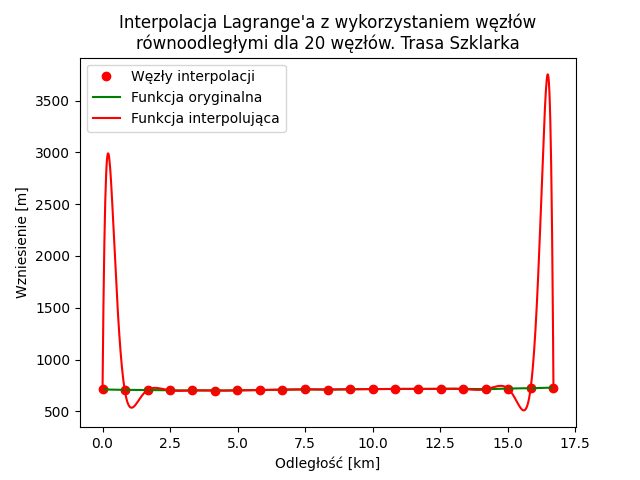
\includegraphics[width=0.5\textwidth]{szklarka_l_r_20.png}}
    \subfloat{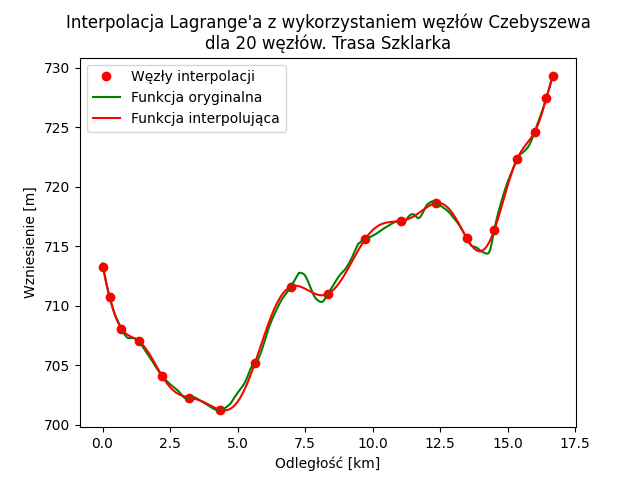
\includegraphics[width=0.5\textwidth]{szklarka_l_c_20.png}}
  \end{figure}
  \begin{figure}[H]
    \centering
    \subfloat{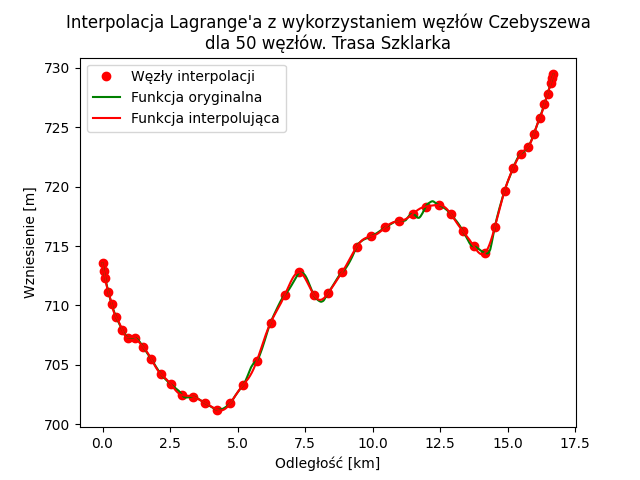
\includegraphics[width=0.5\textwidth]{szklarka_l_c_50.png}}
  \end{figure}

  Tak jak w przypadku pierwszej trasy, interpolacja z użyciem węzłów Czebyszewa daje zadowalające wyniki i zapobiaga
  efektowi Rungego. Dla 50 węzłów, wielomian jest bardzo zbliżony do oryginalnego zbioru punktów.
\end{section}

\begin{section}{Analiza podstawowa interpolacji funkcjami sklejanymi pierwszej trasy}
  \begin{figure}[H]
    \centering
    \subfloat{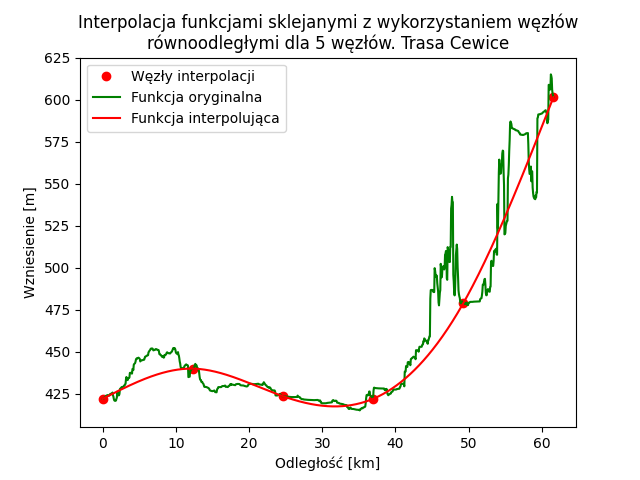
\includegraphics[width=0.5\textwidth]{cewice_f_r_5.png}}
    \subfloat{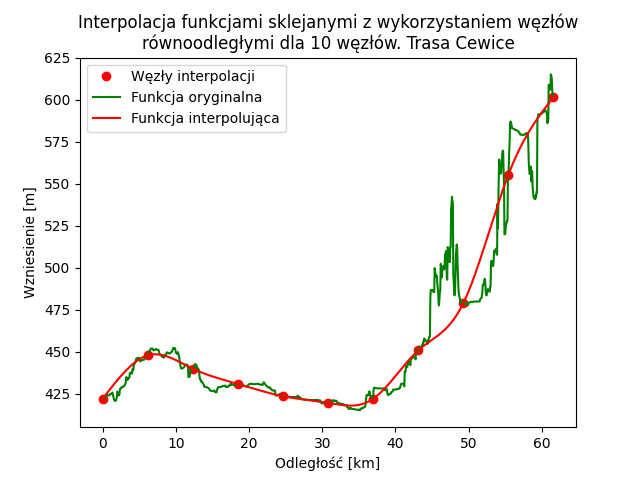
\includegraphics[width=0.5\textwidth]{cewice_f_r_10.png}}
  \end{figure}
  \begin{figure}[H]
    \centering
    \subfloat{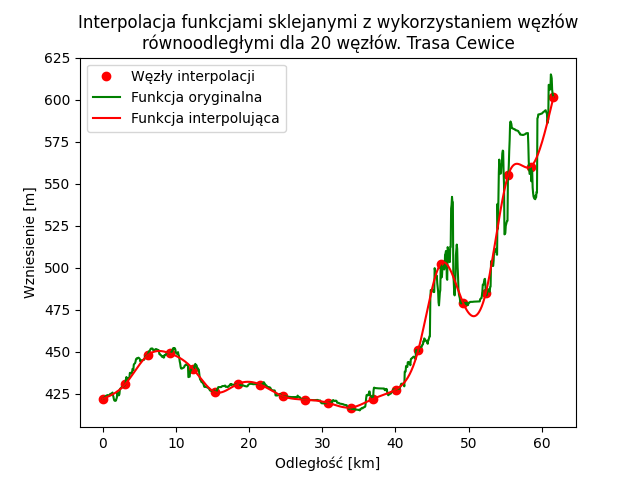
\includegraphics[width=0.5\textwidth]{cewice_f_r_20.png}}
    \subfloat{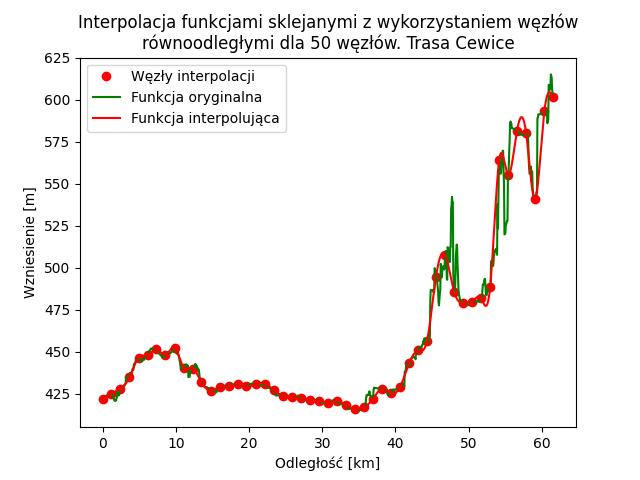
\includegraphics[width=0.5\textwidth]{cewice_f_r_50.png}}
  \end{figure}

  Metoda interpolacji funkcjami sklejanymi daje znacznie lepsze wyniki niż interpolacja wielomianowa. Nie jest podatna na
  efekt Rungego. Jej skuteczność zależy od przebiegu funkcji w każdym podprzedziale, a zatem od liczby węzłów.
\end{section}

\begin{section}{Analiza podstawowa interpolacji funkcjami sklejanymi trzeciej trasy}
  \begin{figure}[H]
    \centering
    \subfloat{\includegraphics[width=0.5\textwidth]{wieżyca_f_r_5.png}}
    \subfloat{\includegraphics[width=0.5\textwidth]{wieżyca_f_r_7.png}}
  \end{figure}
  \begin{figure}[H]
    \centering
    \subfloat{\includegraphics[width=0.5\textwidth]{wieżyca_f_r_15.png}}
    \subfloat{\includegraphics[width=0.5\textwidth]{wieżyca_f_r_50.png}}
  \end{figure}
  \begin{figure}[H]
    \centering
    \subfloat{\includegraphics[width=0.5\textwidth]{wieżyca_l_c_17.png}}
    \subfloat{\includegraphics[width=0.5\textwidth]{wieżyca_l_c_50.png}}
  \end{figure}
  \begin{figure}[H]
    \centering
    \subfloat{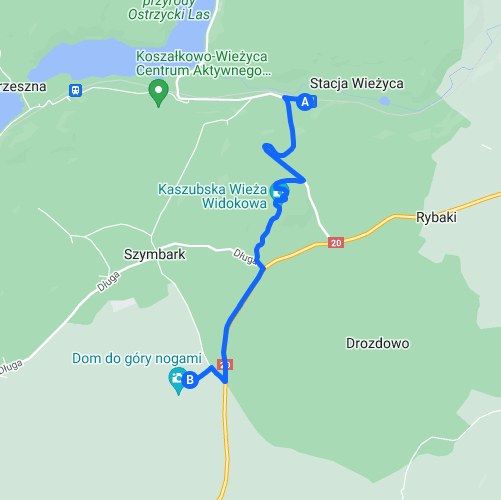
\includegraphics[width=0.5\textwidth]{wiezyca.png}}
  \end{figure}

  Powyżej przedstawiono interpolację trzeciej trasy za pomocą funkcji sklejanych. Funkcje sklejane bardzo dobrze
  radzą sobie z nieregularnościami trasy i nie są podatne na efekt Rungego. Dodatkowo dodałem wykresy dla 17 węzłów
  i 50 węzłów, obliczanych metodą Lagrange'a z użyciem węzłów Czebyszewa. Widać, że na środku przedziału funkcje
  sklejane radzą sobie lepiej, ze względu na charakterystykę węzłów Czebyszewa. Dla 50 węzłów, funkcje sklejane są
  bardzo zbliżone do oryginalnego zbioru punktów.
\end{section}

\begin{section}{Wnioski}
  Interpolacja wielomianowa przy równomiernym rozmieszczeniu węzłów jest podatna na efekt Rungego. Co powoduje 
  niezadowalające wyniki. Interpolacja z użyciem węzłów Czebyszewa pozwala na uniknięcie efektu Rungego, ale
  zwiększa błąd w środku przedziału. Interpolacja funkcjami sklejanymi daje najlepsze wyniki, nie jest podatna na
  efekt Rungego i radzi sobie z nieregularnościami trasy. Dla trasy o dużej liczbie węzłów, interpolacja funkcjami
  daje bardzo dobre wyniki. Dodatkowo interpolacja funkcjami sklejanymi radzi sobie lepiej z dużymi zmianami wartości,
  "ostrymi" wyskokami lub spadkami wartości funkcji.
\end{section}

\begin{section}{Źródła}
  Trasy przygotowane przeze mnie w programie Google Maps. Profile wysokościowe pobrane z przy pomocy Google Maps Elevetion API.
  
  \printbibliography
\end{section}

\end{document}
